\section{Background}
\label{sec:-back}
\subsection{Problem Structure}
The forest coverage classification problem clearly fits into the 
category of a multiclass classification problem, in which we describe 
a classifier that maps from a feature vector to one of a series of 
possible output labels.  This feature vector, as outlined in table 
\ref{table:featurelist}, contains a mix of continuous and discrete 
values.  The discrete features, as visualized in figures \ref{fig:soil} 
and \ref{fig:wilderness}, account for multiclass features encoded with 
the one-hot encoding method.  

Given these features, we wish to classify our example with a choice 
from the labels 
below:
\begin{enumerate}
\item Spruce/Fir
\item Lodgepole Pine
\item Ponderosa Pine
\item Cottonwood/Willow
\item Aspen
\item Douglas-fir
\item Krummholz
\end{enumerate}

Unlike a binary classifier, it is quite easy to end up with an 
error rate well over 50\% when dealing with a multiclass 
classifier.


\begin{figure*}
\centering
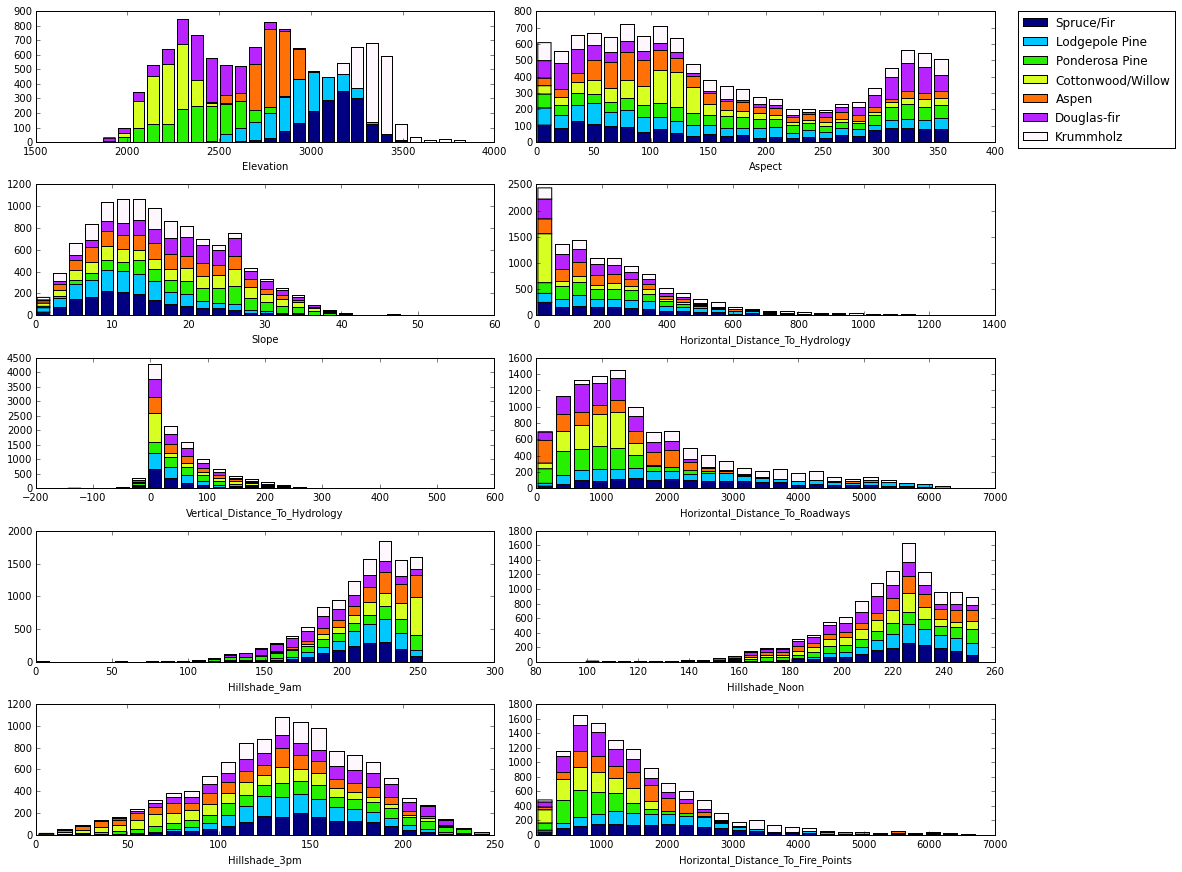
\includegraphics[width=\linewidth]{continuous}
 \caption{Continuous variables}
 \label{fig:continuous_features}
\end{figure*}

\begin{figure*}
\centering
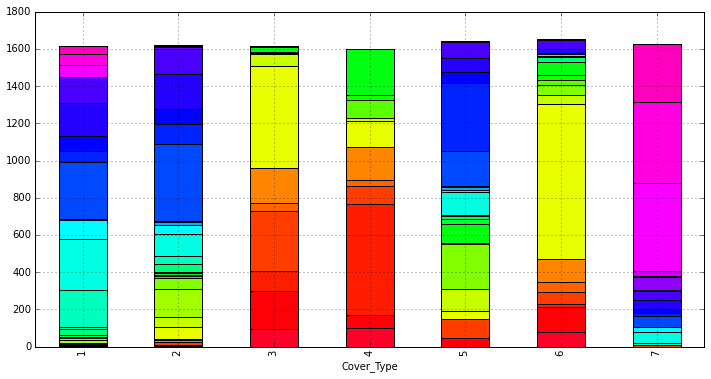
\includegraphics[width=\linewidth]{soil_type}
 \caption{Soil types and accompanying cover types}
 \label{fig:soil}
\end{figure*}

\begin{figure*}
\centering
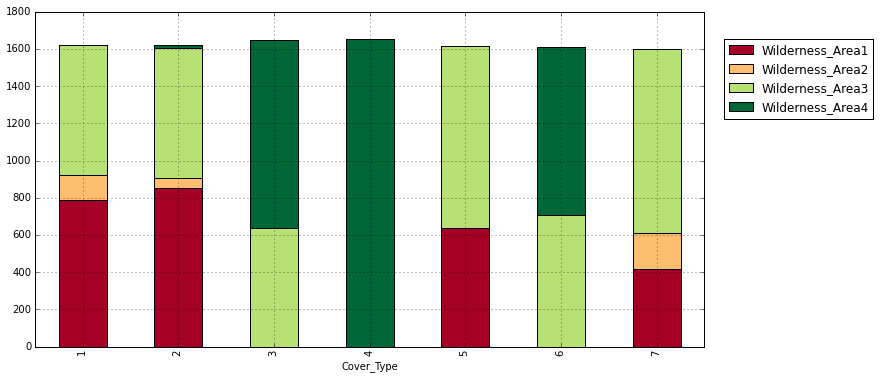
\includegraphics[width=\linewidth]{wilderness}
 \caption{Wilderness types and accompanying cover types}
 \label{fig:wilderness}
\end{figure*}

\subsection{Solution}
The classification solution we assemble to solve this problem involves 
a number of different machine learning models.  We began the project by 
attempting a Random Forest classifier, but eventually expanded to also 
make use of a Gradient Boost Machine, a Support Vector Machine, and a 
k-Nearest Neighbor classifier.  Each of these machines has its own 
strengths and weaknesses, which we will discuss in the following section.


%%% Local Variables: 
%%% mode: latex
%%% TeX-master: "main"
%%% End: 
